\documentclass[8pt]{beamer}

% Beamer style
%\usetheme[secheader]{Madrid}
% \usetheme{CambridgeUS}
\useoutertheme{infolines}
\usecolortheme[rgb={0.65,0.15,0.25}]{structure}
% \usefonttheme[onlymath]{serif}
\beamertemplatenavigationsymbolsempty
%\AtBeginSubsection

% Packages
%\usepackage[french]{babel}
\usepackage[latin1]{inputenc}
\usepackage{color}
\usepackage{xspace}
\usepackage{dsfont, stmaryrd}
\usepackage{amsmath, amsfonts, amssymb}
\usepackage{epsfig}
\usepackage{array}
\usepackage{tikz}
\usepackage{url}
\usepackage{/home/robin/LATEX/Biblio/astats}
%\usepackage[all]{xy}
\usepackage{graphicx}

\input{/home/robin/RECHERCHE/EXPOSES/LATEX/Commands}

% Directory
\newcommand{\fignet}{/home/robin/Bureau/RECHERCHE/RESEAUX/EXPOSES/FIGURES}
\newcommand{\figchp}{/home/robin/Bureau/RECHERCHE/RUPTURES/EXPOSES/FIGURES}


%====================================================================
%====================================================================

%====================================================================
%====================================================================
\begin{document}
%====================================================================
%====================================================================

%====================================================================
\title{Statistical inference of ecological network}

\author[S. Robin]{S. Robin / UMR MIA-Paris / P6}

\institute[INRA / AgroParisTech]{~ \\%INRA / AgroParisTech \\
%   \vspace{-.1\textwidth}
%   \begin{tabular}{ccc}
%     
\includegraphics[height=.06\textheight]{\fignet/LogoINRA-Couleur} & 
%     \hspace{.02\textheight} &
%     
\includegraphics[height=.06\textheight]{\fignet/logagroptechsolo} % & 
%     \hspace{.02\textheight} &
%     
\includegraphics[height=.09\textheight]{\fignet/logo-ssb}
%     \\ 
%   \end{tabular} \\
  \bigskip
  }

\date[NGB, Bordeaux]{Apr. 2018, NGB, Bordeaux}

%====================================================================
%====================================================================
\maketitle
%====================================================================

%====================================================================
\frame{\frametitle{Partner 6}
  \paragraph{UMR MIA-Paris (AgroPArisTech / INRA / univ. Paris-Saclay):}
  \begin{itemize}
   \item Julie Aubert
   \item Julien Chiquet 
   \item Sophie Donnet 
   \item Pierre Barbillon 
   \item Sarah Ouadah 
   \item Maude Delattre 
   \item Emilie Lebarbier 
   \item Raphaelle Momal 
   \item St�phane Robin
  \end{itemize}
  \ra 46 pers. months
}

%====================================================================
%====================================================================
\section{(Ecological) networks}
\frame{\tableofcontents[currentsection]}
%====================================================================
\frame{\frametitle{Ecological networks}

  \begin{tabular}{cc}
    \begin{tabular}{p{.5\textwidth}}
	 \paragraph{Network = graph $G = (V, E)$}
	 \begin{itemize}
	 \item $V =$ set of vertices (or nodes)
	 \item $E =$ set of edges (or links)
	 \end{itemize}
  
	 \bigskip \bigskip \pause
	 \paragraph{Ecological network.}
	 \begin{itemize}
	 \item Nodes = species (or OTU, or taxons)
	 \item Links = interactions between species
	 \end{itemize}
    \end{tabular}
    & 
    \hspace{-.1\textwidth}
    \begin{tabular}{p{.5\textwidth}}
	 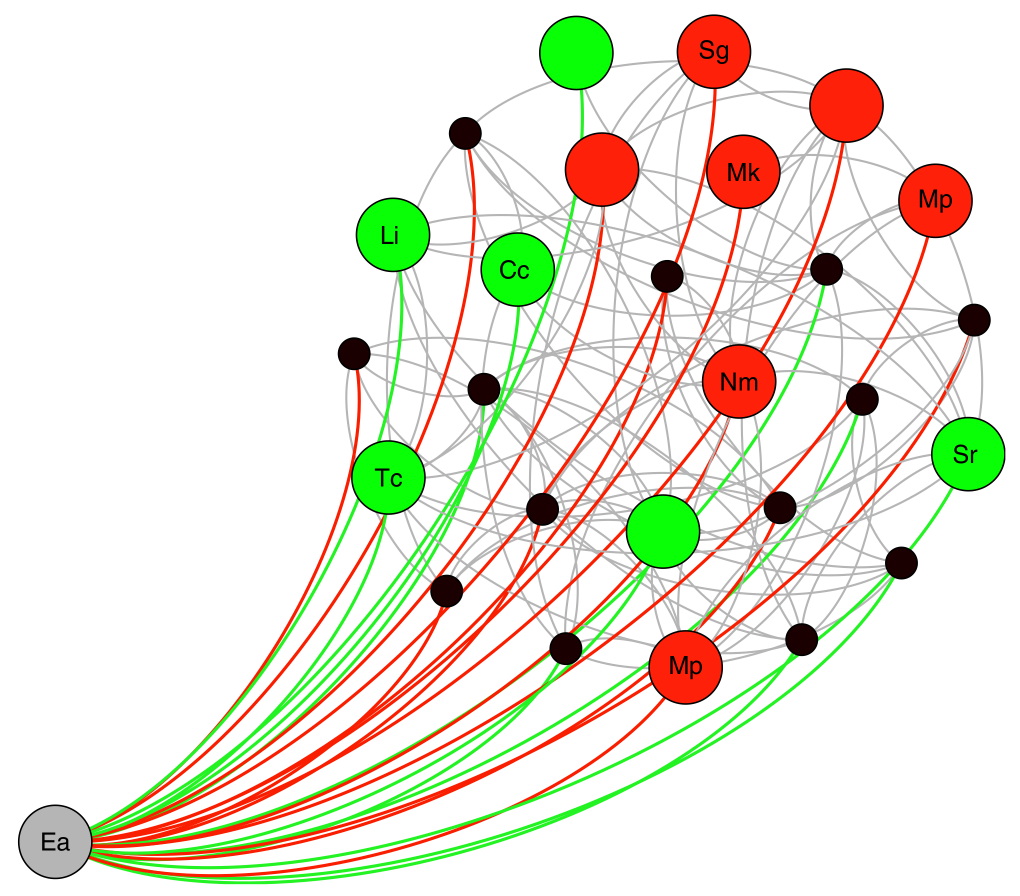
\includegraphics[width=.5\textwidth]{\fignet/JFS16-EnvirMicrobiol-Fig4}
    \end{tabular}
  \end{tabular}
  
  \bigskip \bigskip 
  Edges can be binary ,valued (weighted), univariate or multivariate, etc.
}

%====================================================================
\frame{\frametitle{Statistical analysis of ecological network}

  3 main questions
  
  \bigskip \pause
  \paragraph{Network inference}
  \begin{itemize}
   \item Measures are collected on the nodes (e.g. species 'abundance', NGS read counts)
   \item Statistical question: infer the network based on node measures
  \end{itemize}

  \bigskip \pause
  \paragraph{Network topology} 
  \begin{itemize}
   \item The network is observed
   \item Statistical question: understand its organization (clusters, centrality, diameter, etc)
  \end{itemize}

  \bigskip \pause
  \paragraph{Network as a support}
  \begin{itemize}
   \item The network + measures on the nodes are observed (e.g. spread of an epidemics along the edges of a social network).
   \item Statistical question: understand how the topology of the network influences the dynamic of the process.
  \end{itemize}
}

%====================================================================
%====================================================================
\section{(Ecological) network inference}
\frame{\tableofcontents[currentsection]}
%====================================================================
\frame{\frametitle{Network inference}

  \paragraph{Typical experiment.}
  \begin{itemize}
   \item $i = 1 \dots n$ observations (samples, replicates, dates, \dots)
   \item $j = 1 \dots p$ nodes (species)
   \item $Y = (Y_{ij}) = n\times p$ data matrix ('abundance' of species $j$ in sample $i$)
   \item $X = (x_{ik}) = n \times d$ matrix of covariates describing the experimental conditions for each sample
  \end{itemize}
  
  \bigskip \bigskip \pause
  \paragraph{Statistical approach.}
  \begin{itemize}
   \item The network depicts the relations between the species $(1, \dots j, \dots p)$.
   \item Inferring the network requires to now something about the joint distribution
   $$
   p(Y_i) = p(Y_{i1}, \dots Y_{ij}, \dots Y_{jp})
   $$
   \item A critical issue: there are $2^{p(p-1)/2}$ possible networks\footnote{That is $3.5 \;10^{13}$ for $p=10$, $8.9 \;10^{130}$ for $p = 30$}
  \end{itemize}
}

%====================================================================
\frame{\frametitle{Probabilistic framework: Graphical models}

  \paragraph{Definition \refer{Lau96}.} The joint distribution $p$ is faithful to the graph $G$ 
  $$
  P(Y_1, \dots, Y_p) \propto \prod_{C \in \Ccal_G} \psi_C(Y_C)
  $$
  where $\Ccal_G =$ set of cliques of $G$. % \refer{HaC71}
  
  \bigskip \pause
  \paragraph{Example.} ~ \\
%   \vspace{-.2\textheight}
  \begin{tabular}{cc}
    \begin{tabular}{p{.5\textwidth}}
%     \hspace{-.1\textwidth}
    \includegraphics[width=.4\textwidth]{\fignet/FigGGM-4nodes-red}
    \end{tabular}
    & 
    \hspace{-.05\textwidth}
    \begin{tabular}{p{.4\textwidth}}
    $P(Y_1, Y_2, Y_3, Y_4) \propto$
    $$
    \psi_1(Y_1 ,Y_2, Y_3) \times \psi_2(Y_3, Y_4)
    $$
    
    \bigskip
    $
    \Rightarrow Y_4 \perp (Y_1, Y_2) | Y_3
    $
    \end{tabular}
  \end{tabular} 

  \hspace{-.7\textheight} ~ \pause
  \paragraph{Interpretation.} ~
  \begin{itemize}
  \item Species $4$ is independent from species $1$ and $2$ conditionally on species $3$
  \item The vertices of $G$ only reveal {\sl direct interactions}.
  \end{itemize}
}

%====================================================================
\frame{\frametitle{A nice case: Gaussian graphical models (GGM)}

  \paragraph{Gaussian distribution.}
  $$
  Y_i \sim \Ncal_p(\mu, \Sigma)
  $$
  $\mu =$ vector of means, $\Sigma =$ covariance matrix.
  
  \bigskip \bigskip \pause
  \paragraph{A nice property.} ~ \\
%   \vspace{-.2\textheight}
  \begin{tabular}{cc}
    \begin{tabular}{p{.5\textwidth}}
%     \hspace{-.15\textwidth}
    \includegraphics[width=.4\textwidth]{\fignet/FigGGM-4nodes-red}
    \end{tabular}
    & 
    \hspace{-.15\textwidth}
    \begin{overprint}
    \onslide<2>
    \begin{tabular}{p{.5\textwidth}}
	 Covariance matrix
	 $$
	 \Sigma \propto \left[ \begin{array}{cccc}
	   1 & -.25 & -.41 &  \emphase{.25} \\
	   -.25 &  1 & -.41 &  \emphase{.25} \\
	   -.41 & -.41 &  1 & -.61 \\
	   \emphase{.25} &  \emphase{.25} & -.61 &  1
	   \end{array} \right] 
	 $$
    \end{tabular} 
    \onslide<3>
    \begin{tabular}{p{.5\textwidth}}
	 Inverse covariance matrix
	 $$
	 \Sigma^{-1} \propto \left[ \begin{array}{cccc}
	   1 & .5 & .5 & \emphase{0} \\
	   .5 & 1 & .5 & \emphase{0} \\
	   .5 & .5 & 1 & .5 \\
	   \emphase{0} & \emphase{0} & .5 & 1
	   \end{array} \right] 
	 $$
    \end{tabular} 
    \onslide<4>
    \begin{tabular}{p{.5\textwidth}}
	 Adjacency matrix
	 $$
	 A = \left[ \begin{array}{cccc}
	 0 & 1 & 1 & \emphase{0} \\
	 1 & 0 & 1 & \emphase{0} \\
	 1 & 1 & 0 & 1 \\
	 \emphase{0} & \emphase{0} & 1 & 0 
	 \end{array} \right]
	 $$
    \end{tabular} 
    \onslide<5->
    \begin{tabular}{p{.5\textwidth}}
	 Estimated inverse covariance matrix
	 $$
	 \widehat{\Sigma}^{-1} \propto \left[ \begin{array}{cccc}
	   1 & .48 & .61 & \emphase{.09} \\
	   .48 & 1 & .67 & \emphase{.06} \\
	   .61 & .67 & 1 & .46 \\
	   \emphase{.09} & \emphase{.06} & .46 & 1
	   \end{array} \right] 
	 $$
	 ($n = 100$)
    \end{tabular} 
    \end{overprint}
  \end{tabular}
  
}

%====================================================================
\frame{\frametitle{A popular approach}

  \paragraph{Sparsity assumption:}
  $$
  \Omega = \Sigma^{-1} \text{ is sparse}
  $$
  = most entries of $\Omega$ are zeros.
  
  \bigskip \bigskip \pause
  \paragraph{A series of approaches} for Gaussian data
  \begin{itemize}
   \item Sparse regression of each species on the others:
   $$
   Y_i = a_j + \sum_{j \neq i} b_{ij} Y_j + E_i \quad \text{forcing most $b_{ij} = 0$ \refer{MeB06}}
   $$
   \item Directly estimate $\Omega$ forcing most $\omega_{ij} = 0$ \refer{FHT08} 
   using, e.g, Lasso penalty \refer{Tib96,EHJ04} or more refined \refer{ACM09}.
  \end{itemize}
  
  \bigskip \bigskip \pause
  \paragraph{An important theoretical result \refer{Ver12}.} $k =$ degree of a given node
  \begin{itemize}
  \item $k \log(p/k) \leq n$: \qquad possible recovery of the exact list of neighbors
  \item $k \log(p/k) > n \log n$: impossible recovery of the exact list of neighbors
  \end{itemize}
}

%====================================================================
%====================================================================
\section{Poisson log-normal model}
\frame{\tableofcontents[currentsection]}
%====================================================================
\frame{\frametitle{A multivariate model for abundance data}

  \paragraph{Problem.}
  \begin{itemize}
   \item We need to define a joint distribution for an abundance vector $Y_i = (Y_{i1}, \dots, Y_{ip})$.
   \item It needs to be flexible (no constraints on the sign of correlations \refer{IYA17}).
   \item The Gaussian setting is nice and plenty of tools exist.
   \item But the Gaussian assumption does not hold for abundance data
  \end{itemize}
  
  
  \bigskip \pause
  \ra The Poisson log-normal (PLN) model \refer{AiH89} sees to be a good option.
}

%====================================================================
\frame{\frametitle{Poisson log-normal model}

  \paragraph{Poisson log-normal (PLN) model:} a latent Gaussian model
  \begin{itemize}
   \item $(Z_i)_i:$ iid latent vectors $\sim \Ncal_p(0, \Sigma)$ 
   \item $x_i :$ vector of covariates
   \item $o_i :$ vector of offsets
   \item $Y_i = (Y_{ij})_j:$ counts independent conditional on $Z_i$ 
  $$
  Y_{ij} \,|\, Z_{ij} \sim \Pcal(e^{\emphase{o_{ij} + x_i^\intercal \beta_j} + Z_{ij}})
  $$
  \end{itemize}

  \bigskip \pause
  \paragraph{Interpretation.} 
  \begin{itemize}
   \item Dependency structure encoded in the latent space (i.e. in $\Sigma$)
   \item Additional effects (covariates, offsets) are fixed
   \item Conditional Poisson distribution = noise model
  \end{itemize}
  
  \bigskip \pause
  \paragraph{Our contribution.} Maximum likelihood is difficult for PLN \refer{Kar05} \\
  \ra Variational approximations \refer{WaJ08} allow to circumvent most difficulties.

}

%====================================================================
\frame{\frametitle{A first use of PLN: PCA}

  \paragraph{Dimension reduction.} \refer{CMR17}
  \begin{itemize}
   \item Aim: visualize a large dataset in a reduces dimension
   \item Assumption behind PCA: $\Sigma$ has rank $q < p$
  \end{itemize}

  \bigskip \bigskip \pause
  \paragraph{Pathobiome: Oak powdery mildew.} Data from \refer{JFS16}.
  \begin{itemize}
   \item $n = 116$ oak leaves = samples
   \item $p_1 = 66$ bacterial species (OTU)
   \item $p_2 = 48$ fungal species ($p = 114$)
   \item covariates: tree (resistant, intermediate, susceptible), branch height, distance to trunk, \dots.
   \item offsets: $o_{i1}, o_{i2} =$ offset for bacteria, fungi
  \end{itemize}

}

%====================================================================
\frame{\frametitle{Pathobiome: First 2 PCs}

  On the importance of covariates:
  $$
  \includegraphics[width=.9\textwidth]{../FIGURES/CMR17-Fig1c_IndMap.pdf}
  $$
  \qquad \qquad \qquad offset only \qquad \qquad \qquad \qquad offset + covariates 
}

%====================================================================
\frame{ \frametitle{Network inference with PLN}

  \paragraph{Model:}
  $$
  \text{PLN model}
  \qquad + \qquad
  {\Omega = \Sigma^{-1} \text{ sparse}}
  $$
  
  \bigskip \bigskip \pause
  \paragraph{Interest:} Similar to Gaussian graphical model (GGM) inference

  \bigskip \bigskip \pause
  \paragraph{Sparsity-inducing regularization:} graphical lasso (gLasso, \refer{FHT08})
  $$
  \log p_\theta(Y) - \lambda \; \|\Omega\|_{1, \text{off}}
  $$
  
  \bigskip
  \begin{itemize}
   \item Because of the variational approximation $\log p_\theta(Y)$ is replaced with a lower bound.
  \end{itemize}
}

%====================================================================
\frame{\frametitle{Oak powdery mildew: {\tt PLNmodels} package}

  \paragraph{Syntax:} ~\\ ~
  
  {\tt formula.offset <- Count $\sim$ 1 + offset(log(Offset))} \\~
  
  {\tt models.offset  <- PLNnetwork(formula.offset)} \\~ 

  {\tt best.offset <- models.offset\$getBestModel("BIC")} 

  }

%====================================================================
\frame{\frametitle{Oak powdery mildew: no covariates}

 \bigskip
 {\tt models.offset\$plot()}
 $$
 \includegraphics[height=.7\textheight]{../FIGURES/network_oak_offset_criteria}
 $$
}
 
% %====================================================================
% \frame{\frametitle{Oak powdery mildew: no covariates}
% 
%  \bigskip
%  {\tt best.offset\$plot()}
%  $$
%  \includegraphics[height=.7\textheight]{../FIGURES/network_oak_offset_plot}
%  $$
% }
% 
% %====================================================================
% \frame{\frametitle{Oak powdery mildew: no covariates}
% 
%  \bigskip
%  {\tt best.offset\$plot\_network()}
%  $$
%  \includegraphics[height=.7\textheight]{../FIGURES/network_oak_offset_plot_network}
%  $$
% }
% 
%====================================================================
\frame{\frametitle{Oak powdery mildew: effect of the covariates}

  \begin{tabular}{cc}
   no covariates & covariate = tree + orientation \\
   \begin{tabular}{c}
    \includegraphics[height=.6\textheight]{../FIGURES/network_oak_offset_network}
   \end{tabular}
   &
   \begin{tabular}{c}
    \includegraphics[height=.6\textheight]{../FIGURES/network_oak_tree_or_network}
   \end{tabular}
  \end{tabular}
  
  Ea = {\sl Erysiphe alphitoides} = pathogene responsible for oak mildew
  }


%====================================================================
\frame{ \frametitle{On-going works}

  \paragraph{Around the PLN model.}
  \begin{itemize}
   \item Tree-based network inference (Raphaelle's PhD)
   \item Network comparison
   \item Searching for missing nodes (covariates or species) (\refer{RAR17} + Raphaelle's PhD)
   \item Deal with temporal or spatial data.
   \item Detect changes in the network structure
   \item Be able to assess significance of the covariate effects
  \end{itemize}
  
}

%====================================================================
\frame{ \frametitle{Other network analyses}

  \paragraph{Topological network analyses.}
  \begin{itemize}
   \item Effect of the covariate on the topology of an {\sl observed} network \\
   \ra If needed, try to exhibit a residual structure
   \item Multiplex networks \refer{BDL17} \\
   \ra Dealing with different types of nodes and different types of links
  \end{itemize}

  \bigskip \bigskip 
  \paragraph{Clustering for community ecology.}
  \begin{itemize}
   \item Understand interaction between groups of species and groups of environments 
  \end{itemize}

}

%====================================================================
\frame{ \frametitle{References}
{\tiny
  \bibliography{/home/robin/Biblio/BibGene}
%   \bibliographystyle{/home/robin/LATEX/Biblio/astats}
  \bibliographystyle{alpha}
  }
}

%====================================================================
\appendix 
\section{Appendix}
%====================================================================
\backupbegin
%====================================================================
\frame{\frametitle{PLN network inference}
  
  \renewcommand{\nodesize}{1.75em}
  \renewcommand{\edgeunit}{2.5*\nodesize}
  \paragraph{Cheat:} Use the PLN model and infer the graphical model of $Z$
  
  \bigskip  
  \begin{overprint}
   \onslide<2>
    $$
    \begin{array}{ccc}
    {\footnotesize \begin{tikzpicture}
\node[hidden] (Z1) at ( 0.95*\edgeunit,  0.31*\edgeunit) {$Z_1$};
\node[hidden] (Z2) at (-0.00*\edgeunit,  1.00*\edgeunit) {$Z_2$};
\node[hidden] (Z3) at (-0.95*\edgeunit,  0.31*\edgeunit) {$Z_3$};
\node[hidden] (Z4) at (-0.59*\edgeunit, -0.81*\edgeunit) {$Z_4$};
\node[hidden] (Z5) at ( 0.59*\edgeunit, -0.81*\edgeunit) {$Z_5$};

\draw[edge] (Z1) to (Z5);  \draw[edge] (Z2) to (Z3);  
\draw[edge] (Z2) to (Z4);  \draw[edge] (Z3) to (Z4); 

\node[observed] (Y1) at ( 1.05*\edgeunit, -0.39*\edgeunit) {$Y_1$};
\node[observed] (Y2) at (-0.00*\edgeunit,  0.30*\edgeunit) {$Y_2$};
\node[observed] (Y3) at (-1.05*\edgeunit, -0.39*\edgeunit) {$Y_3$};
\node[observed] (Y4) at (-0.59*\edgeunit, -1.51*\edgeunit) {$Y_4$};
\node[observed] (Y5) at ( 0.59*\edgeunit, -1.51*\edgeunit) {$Y_5$};

\draw[arrow] (Z1) to (Y1); 
\draw[arrow] (Z2) to (Y2);
\draw[arrow] (Z3) to (Y3);
\draw[arrow] (Z4) to (Y4);
\draw[arrow] (Z5) to (Y5);
\end{tikzpicture}
 }
    & \qquad &
    {\footnotesize \begin{tikzpicture}
\node[observed] (Y1) at ( 0.95*\edgeunit,  0.31*\edgeunit) {$Y_1$};
\node[observed] (Y2) at (-0.00*\edgeunit,  1.00*\edgeunit) {$Y_2$};
\node[observed] (Y3) at (-0.95*\edgeunit,  0.31*\edgeunit) {$Y_3$};
\node[observed] (Y4) at (-0.59*\edgeunit, -0.81*\edgeunit) {$Y_4$};
\node[observed] (Y5) at ( 0.59*\edgeunit, -0.81*\edgeunit) {$Y_5$};

\node[empty] (YY) at ( 0.59*\edgeunit, -1.51*\edgeunit) {};

\draw[edge] (Y1) to (Y5);  \draw[edge] (Y2) to (Y3);  
\draw[edge] (Y2) to (Y4);  \draw[edge] (Y3) to (Y4);  
\end{tikzpicture}    
 }
    \end{array}
    $$
  \onslide<3>
   $$
   \begin{array}{ccc}
   {\footnotesize \begin{tikzpicture}
\node[hidden] (Z1) at ( 0.95*\edgeunit,  0.31*\edgeunit) {$Z_1$};
\node[hidden] (Z2) at (-0.00*\edgeunit,  1.00*\edgeunit) {$Z_2$};
\node[hidden] (Z3) at (-0.95*\edgeunit,  0.31*\edgeunit) {$Z_3$};
\node[hidden] (Z4) at (-0.59*\edgeunit, -0.81*\edgeunit) {$Z_4$};
\node[hidden] (Z5) at ( 0.59*\edgeunit, -0.81*\edgeunit) {$Z_5$};

\draw[edge] (Z1) to (Z2);  \draw[edge] (Z1) to (Z4);  
\draw[edge] (Z1) to (Z5);  \draw[edge] (Z2) to (Z3);  
\draw[edge] (Z2) to (Z4);  \draw[edge] (Z3) to (Z4); 

\node[observed] (Y1) at ( 1.05*\edgeunit, -0.39*\edgeunit) {$Y_1$};
\node[observed] (Y2) at (-0.00*\edgeunit,  0.30*\edgeunit) {$Y_2$};
\node[observed] (Y3) at (-1.05*\edgeunit, -0.39*\edgeunit) {$Y_3$};
\node[observed] (Y4) at (-0.59*\edgeunit, -1.51*\edgeunit) {$Y_4$};
\node[observed] (Y5) at ( 0.59*\edgeunit, -1.51*\edgeunit) {$Y_5$};

\draw[arrow] (Z1) to (Y1); 
\draw[arrow] (Z2) to (Y2);
\draw[arrow] (Z3) to (Y3);
\draw[arrow] (Z4) to (Y4);
\draw[arrow] (Z5) to (Y5);
\end{tikzpicture}
 }
   & \qquad &
   {\footnotesize \begin{tikzpicture}
\node[observed] (Y1) at ( 0.95*\edgeunit,  0.31*\edgeunit) {$Y_1$};
\node[observed] (Y2) at (-0.00*\edgeunit,  1.00*\edgeunit) {$Y_2$};
\node[observed] (Y3) at (-0.95*\edgeunit,  0.31*\edgeunit) {$Y_3$};
\node[observed] (Y4) at (-0.59*\edgeunit, -0.81*\edgeunit) {$Y_4$};
\node[observed] (Y5) at ( 0.59*\edgeunit, -0.81*\edgeunit) {$Y_5$};

\node[empty] (YY) at ( 0.59*\edgeunit, -1.51*\edgeunit) {};

\draw[edge] (Y1) to (Y2);  \draw[edge] (Y1) to (Y3);  
\draw[edge] (Y1) to (Y4);  \draw[edge] (Y1) to (Y5);  
\draw[edge] (Y2) to (Y3);  \draw[edge] (Y2) to (Y4); 
\draw[edge] (Y2) to (Y5);  \draw[edge] (Y3) to (Y4);  
\draw[edge] (Y3) to (Y5);  \draw[edge] (Y4) to (Y5);  
\end{tikzpicture} }
   \end{array}
  $$
  \end{overprint}

  \bigskip
  \onslide+<3->{
  $$
  \text{Graphical model of $Z$ \emphase{$\neq$} Graphical model of $Y$}
  $$
  }
}

%====================================================================
\frame{\frametitle{Changes in network structure} 

  \paragraph{Gene expression in {\sl Drosophila}:} $N = 67$ time points, $p = 11$ genes, four expected regions

  \pause \bigskip
  Posterior probability of change-points \refer{ScR16}:
  $$
  \includegraphics[width=.7\textwidth]{\figchp/ScR16-Fig8-chgpt_EMP_ap10_au1}
  $$
  \pause
  Inferred networks:
  $$
  \includegraphics[width=.8\textwidth]{\figchp/ScR16-Fig9-network_seuil02}
  $$
}

%====================================================================
\frame{\frametitle{Effect of covariate on a network structure}

  \paragraph{Tree species interaction network}
  $n = 51$ species ($N = 1275$ pairs), 3 covariates (phylogenetic, taxonomic \& geographical  distance), density $= .54$ (data from \refer{VPD08})

  \bigskip
  \begin{tabular}{cc}
    \begin{tabular}{p{.5\textwidth}}
	 Inferred graphon (no covariate) \\ ~\\
	 \includegraphics[height=.4\textheight]{\fignet/treed0} \\ ~\\
	 ~
    \end{tabular}
    & 
    \hspace{-.05\textwidth}
    \begin{tabular}{p{.5\textwidth}}
	 Residual graphon (3 covariates) \\ ~\\
	 \includegraphics[height=.4\textheight]{\fignet/treed3} \\ ~\\
	 $P(H_0) \simeq 10^{-115}$
    \end{tabular}
  \end{tabular}
  
  \refer{LaR16,LRO17}
  }

%====================================================================
%====================================================================
\backupend
%====================================================================

%====================================================================
%====================================================================
\end{document}
%====================================================================
%====================================================================

  \begin{tabular}{cc}
    \begin{tabular}{p{.5\textwidth}}
    \end{tabular}
    & 
    \hspace{-.02\textwidth}
    \begin{tabular}{p{.5\textwidth}}
    \end{tabular}
  \end{tabular}
